\frontmatter % Use roman page numbering style (i, ii, iii, iv...) for the pre-content pages

\pagestyle{plain} % Default to the plain heading style until the thesis style is called for the body content

%----------------------------------------------------------------------------------------
%	TITLE PAGE
%----------------------------------------------------------------------------------------

\begin{titlepage}
\begin{center}

\vspace*{.02\textheight}
%{\scshape\LARGE \univname\par}\vspace{1.5cm} % University name
% \bigskip  
%\textsc{\Large Doctoral Thesis}\\[0.5cm] % Thesis type

%\HRule \\[0.4cm] % Horizontal line

%{\huge \bfseries \ttitle\par}\vspace{0.6cm} % Thesis title automatic

{\bfseries
\LARGE{The Origin and Evolution of Life on a Pale Blue Dot}\\
\bigskip
\large{Astrophysical, Geochemical and Biological Constraints on Habitability}
}

\vspace{1cm} % Thesis title

%\HRule \\[1.2cm] % Horizontal line
 
\begin{minipage}[t]{0.3\textwidth}
\begin{center}
 \large
%\emph{Author:}\\
 \authorname % Author name - remove the \href bracket to remove the link
\end{center}
\end{minipage}

%\begin{minipage}[t]{0.4\textwidth}
%\begin{flushright} \large
%\emph{Supervisor:} \\
%\href{http://www.jamessmith.com}{\supname} % Supervisor name - remove the \href bracket to remove the link  
%\end{flushright}
%\end{minipage}\\[3cm]
 
\vspace{1cm}
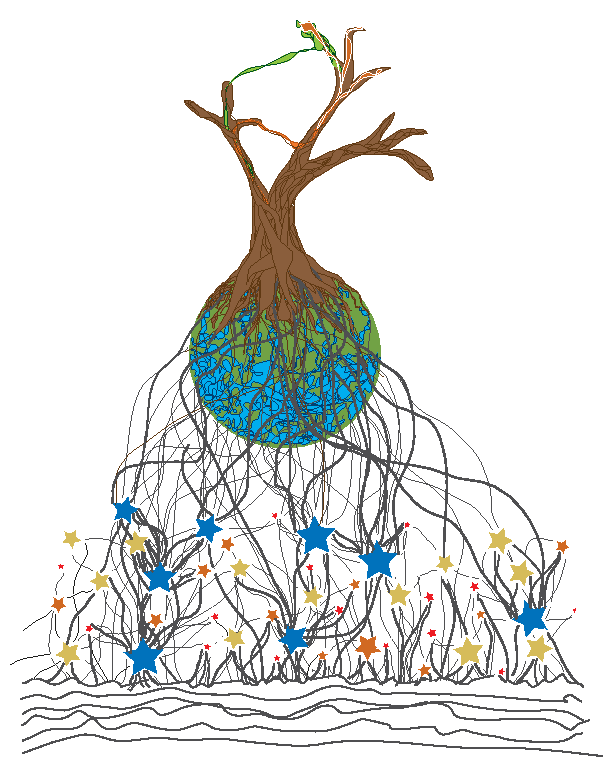
\includegraphics[width=0.6\textwidth]{gfx/front_cover} \\ \bigskip  
\vspace{1cm}

\large \textit{A thesis submitted for the degree of \degreename}\\[0.7cm] % University requirement text
%\textit{in the}\\[0.4cm]
\groupname\\
\deptname\\ % Research group name and department name
%\univname % University name

%{\small Draft (\today)}\\[2cm] % Date
%\includegraphics{Logo} % University/department logo - uncomment to place it


\includegraphics[width=5cm]{gfx/ANU_LOGO_cmyk_56mm}

{\normalsize November, 2015}\\[2cm] % Date

\end{center}
\end{titlepage}

%----------------------------------------------------------------------------------------
%	DECLARATION PAGE
%----------------------------------------------------------------------------------------

\begin{declaration}
%\addchaptertocentry{\authorshipname} % Add the declaration to the table of contents
\begingroup
\large
\noindent This dissertation is an account of research undertaken between April 2009 and November 2015 at the Research School of Earth Sciences, The Australian National University, Canberra, Australia. 

%Except where acknowledged in the customary manner, all material presented in this dissertation including figures and photographs are original and have not been submitted in whole or part for a degree in any university.

The work presented in this thesis is that of the candidate alone, except where indicated by due literature reference and acknowledgements in the text. It has not been submitted in whole or in part for any other degree at this or any other university.

This thesis is based on six papers published in refereed scientific journals or books. The development of ideas and research was undertaken with guidance from my supervisor Charles H. Lineweaver and published papers presented in the thesis were written collaboratively with him. Below I describe my contributions to the research in each chapter and associated papers.

\begin{itemize}
\item Chapter~\ref{ch:HabitableWorlds} is the paper \citet{Lineweaver2012AnnRev}. Section~\ref{sec:HZones} is my major research contribution to the paper. Research on the distribution of biomass on Earth, the constraints for habitable zones within the Earth, and the energy requirements and sources for the earliest bacteria is my work.
\item Chapter~\ref{ch:biologicalhab} is the paper \citet{Chopra2016} where my research forms a major contribution to all sections of the paper.
\end{itemize}


\bigskip
\vspace{1cm}
\begin{flushright}
\authorname\\
\today
\end{flushright}
\endgroup
\end{declaration}
\vspace{3cm}
\begingroup
\footnotesize\emph{{Cover: Figure 1 from \fullcite{Lineweaver2012AnnRev}}}
\endgroup
\cleardoublepage

% \begin{declaration}
% \addchaptertocentry{\authorshipname} % Add the declaration to the table of contents
% \noindent I, \authorname, declare that this thesis titled, \enquote{\ttitle} and the work presented in it are my own. I confirm that:

% \begin{itemize} 
% \item This work was done wholly or mainly while in candidature for a research degree at this University.
% \item Where any part of this thesis has previously been submitted for a degree or any other qualification at this University or any other institution, this has been clearly stated.
% \item Where I have consulted the published work of others, this is always clearly attributed.
% \item Where I have quoted from the work of others, the source is always given. With the exception of such quotations, this thesis is entirely my own work.
% \item I have acknowledged all main sources of help.
% \item Where the thesis is based on work done by myself jointly with others, I have made clear exactly what was done by others and what I have contributed myself.\\
% \end{itemize}
 
% \noindent Signed:\\
% \rule[0.5em]{25em}{0.5pt} % This prints a line for the signature
 
% \noindent Date:\\
% \rule[0.5em]{25em}{0.5pt} % This prints a line to write the date
% \end{declaration}

% \cleardoublepage

%----------------------------------------------------------------------------------------
%	QUOTATION PAGE
%----------------------------------------------------------------------------------------

% \vspace*{0.2\textheight}

% \noindent\enquote{\itshape Thanks to my solid academic training, today I can write hundreds of words on virtually any topic without possessing a shred of information, which is how I got a good job in journalism.}

% \hfill Dave Barry

%----------------------------------------------------------------------------------------
%	ACKNOWLEDGEMENTS
%----------------------------------------------------------------------------------------

\begin{acknowledgements}
\addchaptertocentry{\acknowledgementname} % Add the acknowledgements to the table of contents
\vspace{0.4cm}
\begingroup
\normalsize
Like Sagan's apple pie, this thesis was not put together from scratch, because that would have required me to first create the universe. So to all baryons, wise ancestors and enlightened cousins, eukaryotic or otherwise, thank you.

I am grateful to my supervisor, research school, friends and family.

Thank you Google et al. May the electrons keep following and the entropy keep increasing\dots
\endgroup
\end{acknowledgements}

%----------------------------------------------------------------------------------------
%	ABSTRACT PAGE
%----------------------------------------------------------------------------------------

\begin{abstract}
\addchaptertocentry{\abstractname} % Add the abstract to the table of contents
\begingroup
\normalsize
Some of the most fundamental questions in astrobiology are: How does life begin and evolve\,? Does life exist elsewhere in the universe\,? What is the future of life on Earth and beyond\,? This thesis approaches these questions by investigating the chemical and energy requirements for life and the conditions that enabled the emergence and proliferation of life on Earth. Understanding how common the necessary physical processes, chemical ingredients and environmental conditions may be on other planets helps us assess the likelihood of finding life beyond our planet and gives us clues about the best targets and detection methods for future search efforts.

Our evaluation of astrophysical and geochemical constraints on the habitability of Earth-like planets tells us that temperature and the presence of water are the main factors that define the limits for life. Our analysis of recent exoplanet detections suggests that the fraction of stars with planets is $\sim$\,100\%, and that the fraction with wet rocky planets is likely to be comparably large. We find that the most fundamental free energy redox and photon gradients associated with the earliest life forms on Earth, and the energy-transducing metabolisms they induce, are plausible on other wet rocky planets.

Even if the emergence of life is a common feature of planetary systems throughout the universe, we propose a new Gaian bottleneck hypothesis where we postulate that in addition to water, energy and abiogenesis, the early extinction of planetary life is also a cosmic imperative. We discuss why the vast majority of initially wet rocky planetary environments evolve away from habitable conditions within about a billion years because of the strength, rapidity and universality of abiotic positive feedbacks in the atmospheres of terrestrial planets in traditional circumstellar habitable zones. We argue that the maintenance of planetary habitability is a property more associated with an unusually rapid evolution of biological regulation of surface volatiles, than with the luminosity and distance to the host star. Our model suggests that a planet needs to be inhabited in order to remain habitable and predicts that lifeless habitable planets will be rare. The Gaian bottleneck to the long-term persistence of life may be a better explanation for the non-prevalence of extraterrestrial life than the conventional emergence bottleneck paradigm.
\bigskip

\textbf{Keywords:} \keywordnames

\endgroup
\end{abstract}

%----------------------------------------------------------------------------------------
%	LIST OF CONTENTS/FIGURES/TABLES PAGES
%----------------------------------------------------------------------------------------

\renewcommand{\listfigurename}{Figures}
\renewcommand{\listtablename}{Tables}

\begin{spacing}{0.94} 
\tableofcontents % Prints the main table of contents
\end{spacing}

\listoffigures % Prints the list of figures
\listoftables % Prints the list of tables
% \listoflistings % Prints the list of python codes

%----------------------------------------------------------------------------------------
%	ABBREVIATIONS
%----------------------------------------------------------------------------------------

\begin{abbreviations}{ll} % Include a list of abbreviations (a table of two columns)
\textbf{ANU}&\textbf{A}ustralian \textbf{N}ational \textbf{U}niversity\\
\textbf{BOM}&\textbf{B}ureau of \textbf{M}eteorology\\
\textbf{CSIRO}&\textbf{C}ommonwealth \textbf{S}cientific and \textbf{I}ndustrial \textbf{R}esearch \textbf{O}rganisation\\
\textbf{LAH} & \textbf{L}ist \textbf{A}bbreviations \textbf{H}ere\\
\textbf{WSF} & \textbf{W}hat (it) \textbf{S}tands \textbf{F}or\\
\end{abbreviations}

%----------------------------------------------------------------------------------------
%	PHYSICAL CONSTANTS/OTHER DEFINITIONS
%----------------------------------------------------------------------------------------

\begin{constants}{lr@{${}={}$}l} % The list of physical constants is a three column table

% The \SI{}{} command is provided by the siunitx package, see its documentation for instructions on how to use it

Speed of Light & $c_{0}$ & \SI{2.99792458e8}{\meter\per\second} (exact)\\
%Constant Name & $Symbol$ & $Constant Value$ with units\\

\end{constants}

%----------------------------------------------------------------------------------------
%	SYMBOLS
%----------------------------------------------------------------------------------------

\begin{symbols}{lll} % Include a list of Symbols (a three column table)

$a$ & distance & \si{\meter} \\
$P$ & power & \si{\watt} (\si{\joule\per\second}) \\
%Symbol & Name & Unit \\

\addlinespace % Gap to separate the Roman symbols from the Greek

$\omega$ & angular frequency & \si{\radian} \\

\end{symbols}

%----------------------------------------------------------------------------------------
%	DEDICATION
%----------------------------------------------------------------------------------------

\dedicatory{For/Dedicated to/To my\ldots} 


